\documentclass[11pt]{article}

\usepackage[T1]{fontenc}
\usepackage[utf8]{inputenc}
\usepackage{lmodern}
\usepackage[margin=1in]{geometry}
\usepackage{microtype}
\usepackage{booktabs}
\usepackage{graphicx}
\usepackage{amsmath}
\usepackage{hyperref}
\usepackage{xcolor}
\usepackage{enumitem}
\usepackage{caption}

\hypersetup{
  colorlinks=true,
  linkcolor=blue!50!black,
  citecolor=blue!50!black,
  urlcolor=blue!50!black,
}

\title{Latent Cost Repair for World-Model-Based Planning:\\A Cost-Side Fix for an Undertrained LeWorldModel}
\author{Wally Project\\Technical Report}
\date{\today}

\begin{document}
\maketitle

\begin{abstract}
\noindent
Wally is a Minecraft AI research project that trains a LeWorldModel-style
latent dynamics world model and plans actions via CEM-based MPC. A
1{,}000-step L0 checkpoint (ViT-Tiny encoder, 6-layer Transformer
predictor with AdaLN action conditioning, 64$\times$64 frames)
exhibits a 1-D, brightness-dominated latent and a non-monotonic camera
response, so the planner shakes the view without making progress
toward the goal. We diagnose six concrete failures, apply six
cost-side repairs (180$\times$ camera-scale fix, cosine-distance cost,
disabled planner penalties, per-step camera clamp + EMA,
$replan\_interval = 2$, and a TRM reachability head trained on
same-episode temporal separations), and evaluate the planning signal
with the same-candidate selection audit (SCSA) from the TRM paper.
The TRM head lifts the per-replan ranking agreement between the
planner's hybrid cost and the latent-L2 diagnostic from
Spearman $+0.308$ to $+0.924$ and drops the median oracle-best rank
from the 27th to the 2.4th percentile, exceeding the TRM paper's
TwoRoom result ($+0.729$). Despite this, agent behavior does not
improve: the 1k L0's brightness axis is a structural ceiling, and a
better cost function cannot choose tree-look frames the encoder has
never learned to represent. We treat the experiment as the TRM
paper's ``PushT boundary case'' and ship the head ready to use on
the 5k retrain.
\end{abstract}

\section{Introduction}
\label{sec:intro}

Wally trains a LeWorldModel-style latent dynamics world model on
Minecraft trajectories and plans actions via CEM-based MPC, all on a
single AMD RX 6700 XT using Windows-native ROCm. The training
pipeline, the agent loop, and the data format are documented
in~\cite{wally:ag, wally:root}. Reference papers on the LeWorldModel
architecture~\cite{lewm} and the FF-JEPA framework for frozen
encoders~\cite{ffjepa} are at the repo root.

This technical report documents a \emph{cost-side} repair effort on
the 1{,}000-step L0 checkpoint at
\texttt{checkpoints/wood\_1000/checkpoint\_1000.pt} (vit\_tiny,
depth=4, \texttt{encoder\_type=cnn}, \texttt{embed\_dim}=192). After
1k steps the model is not yet a useful dynamics engine, but it is
also not noise: the latent is informative at the frame-pair level
(Spearman $+0.84$ with pixel L2 over 1{,}024 pairs) and a toy
2-D CEM loop on a synthetic positional encoder succeeds at
$77\% / 0.15$ in H=20. The bulk of the failures are therefore on the
\emph{cost side} (camera scale, latent geometry, planner penalties)
plus one \emph{dynamics-side} repair (camera clamp) and one
\emph{learned cost} (TRM reachability head) that fixes the
ranking/trap problem the paper documents in Section~\ref{sec:scsa}.

We make three concrete contributions. (i)~A clean diagnosis of the
1k L0 from twelve 100--200-line probe scripts. (ii)~Six cost-side
repairs, each implemented, tested, and confirmed not to regress
existing behaviour. (iii)~A TRM reachability head integrated into
the CEM planner and a published SCSA result of $+0.924$ mean Spearman
on a 300-replan, 64-population audit. The paper is honest about the
limit: the head is necessary, but on a 1-D latent it is not
sufficient. We treat this as a PushT boundary case and ship the head
to the next retrain.

The paper is structured as: background on the model and planner
(Section~\ref{sec:background}), the diagnosed failures
(Section~\ref{sec:failures}), the repairs (Section~\ref{sec:repairs}),
the SCSA audit (Section~\ref{sec:scsa}), the TRM head itself
(Section~\ref{sec:trm}), results (Section~\ref{sec:results}),
discussion (Section~\ref{sec:discussion}), and reproducibility
(Section~\ref{sec:repro}).

\section{Background}
\label{sec:background}

\textbf{LeWorldModel architecture.}
The L0 is a ViT-Tiny (depth 4, 192-dim) CNN encoder, a 2-layer
projector, an AdaLN-Zero 6-layer Transformer predictor, and a
Softplus + LayerNorm head. Actions enter as a separate conditioning
sequence $c_t$ and modulate the predictor via
$\gamma_t, \beta_t = \mathrm{MLP}(c_t)$. The loss is
$L = \|\hat{z}_{t+1} - z_{t+1}\|^2 + 0.1 \cdot \mathrm{SIGReg}$,
matching the LeWorldModel paper. The full layout is in
\texttt{src/wally/models/}; the AdaLN-Zero design and the SIGReg
application point match the upstream
\texttt{lucas-maes/le-wm}~\cite{lewm} and the FF-JEPA framing
for frozen encoders~\cite{ffjepa}.

\textbf{CEM-based MPC.}
A \texttt{GoalConditionedPlanner} (\texttt{src/wally/planner/plan.py})
encodes the current frame and the goal frame through the L0 encoder,
then runs cross-entropy method optimisation
(\texttt{src/wally/planner/cem.py}) over a population of $H$-step
action sequences to minimise a hybrid cost
$\hat c = c_{\mathrm{lat}}(z_H, z_g) + c_{\mathrm{penalties}}$.
$z_H$ is the predictor's last latent after the rollout. The agent
loop (\texttt{src/wally/agent/loop.py}) re-plans every
\texttt{replan\_interval} steps and warm-starts the next plan by
shifting the previous mean by one window.

\textbf{The latent-proximity trap.}
A latent cost can be predictive \emph{on average} over many
frame-pairs but expose the wrong candidate ordering at each
individual decision. The TRM paper formalises this and proposes a
pairwise reachability head
$m_\phi(z_i, z_j) \in \mathbb R_+$ trained on same-episode temporal
separations $y_{ij} = |t_i - t_j|$, combined with the latent cost
via the hybrid standardisation of Eq.~(6):
\begin{equation}
c_{\mathrm{hyb}}
  = \frac{c_{\mathrm{lat}} - \mu_{\mathrm{lat}}}{\sigma_{\mathrm{lat}}}
  + \lambda \cdot \frac{m_\phi(z_H, z_g) - \mu_\phi}{\sigma_\phi}.
  \label{eq:hybrid}
\end{equation}
The TRM paper's SCSA (App.~B.1) is the standard way to measure
whether $c_{\mathrm{lat}}$ and $m_\phi$ agree on which CEM
candidate to pick.

\section{Diagnosed failures}
\label{sec:failures}

We ran twelve probe scripts against the frozen 1k L0
(\texttt{tools/experiments/00\_...07\_*.py}, 6 figures; full
report in~\cite{wally:report}). The summary:

\begin{enumerate}[leftmargin=*,itemsep=2pt]
\item \textbf{1-D brightness latent.}
PC1 captures $84\%$ of variance; $\|\hat z\|$ correlates with
frame brightness at $+0.97$ and sky-fraction at $+0.92$
(\texttt{04\_latent\_geometry.py}; see
\texttt{\_figures/04\_norm\_vs\_brightness.png}). The CNN encoder
has not learned any spatial structure beyond ``how bright is the
upper half of the frame''.

\item \textbf{Non-monotonic camera response.}
The predictor's one-step $\| \Delta z \|$ on a single camera action
peaks at $|\mathrm{cam}| \approx 0.2$ (yaw $\Delta z = 3.0$, MSE
$10.7$) and falls to MSE $2.6$ at $|\mathrm{cam}| = 1.0$
(\texttt{03\_camera\_shake\_sandbox.py}). The action embedder
amplifies camera inputs by 11$\times$ when the planner sends
$|\mathrm{cam}|=1.0$ (\texttt{01\_ood\_probe.py} C-section).

\item \textbf{8-step rollouts on the edge of the training
distribution.} 100 random rollouts per start, H=8, mean
$\|z_H\| = 8.77$ vs training mean $7.43$ -- $1.3\sigma$ above
(\texttt{02\_rollout\_divergence.py}). Faster replanning does not
help because the 8-step rollout is already marginal.

\item \textbf{OOD cost spikes.}
Synthesised sky/water frames are $35$--$100\times$ further from
training latents than the worst-case real frame; 1-step prediction
error on a synth sky target is $873$ vs $25$ for real
(\texttt{01\_ood\_probe.py}).

\item \textbf{The planner is fine.}
Toy 2-D world with a deterministic Fourier-feature positional
encoder + perfect MLP WM: CEM(H=20, pop 128, iters 10) hits
$77\%$ success at distance $0.15$ (\texttt{06c\_toy\_2d\_world\_positional.py}).
The earlier 06 / 06b toy attempts failed for unrelated reasons
(frozen Minecraft encoder is noise on toy images; jointly-trained
CNN encoder collapsed).

\item \textbf{L0 cost is informative but coarse.}
Spearman $+0.84$ with pixel L2 over 1{,}024 frame pairs; top-1
nearest-by-cost vs nearest-by-pixel agreement $75\%$
(\texttt{07\_cost\_informativeness.py}). The remaining $25\%$
mismatch is dominated by the brightness axis.
\end{enumerate}

Each of these maps to a specific repair.

\section{Cost-side repairs}
\label{sec:repairs}

\subsection{Camera scale fix (180$\times$)}

The L0 is trained on actions clamped to $[-1, 1]$ by the data
loader~\cite{wally:ag} (the raw training data has camera deltas
in degrees, observed range $-42$ to $+37$, which destabilises the
predictor transformer -- the loader clamps to $\pm 1$). The
planner was rescaling camera actions by $180$ before sending
them to the L0, producing L0 inputs up to $\pm 180$ -- an
$11\times$ extrapolation through the action embedder that never
appeared in training.

The fix at \texttt{src/wally/planner/rollout.py:122} is a one-line
change:
\begin{verbatim}
_CAMERA_DEGREE_SCALE: float = 1.0    # was 180.0
\end{verbatim}
The env at \texttt{src/wally/agent/env.py:94,98} still rescales
the agent's $[-1, 1]$ camera to degrees for MineStudio; only the
L0's input stops being multiplied.

\subsection{Cosine-distance cost}

Replace the raw L2 cost
$\|z_H - z_g\|^2$ in
\texttt{src/wally/planner/plan.py:13--32} with the standard cosine
distance on the unit-normalised latents:
\begin{equation}
c_{\mathrm{lat}}(z_H, z_g) = \left\|
  \tfrac{z_H}{\|z_H\| + \epsilon}
  - \tfrac{z_g}{\|z_g\| + \epsilon}
\right\|^2,\quad \epsilon = 10^{-6}.
\label{eq:cosine}
\end{equation}
The cost is bounded in $[0, 4]$ and is equivalent to
$2(1 - \cos\angle(z_H, z_g))$. The brightness dim is still
present (cosine does not normalise across dimensions), but
\emph{content} dims (PC2+) get equal weight per dim.

\subsection{Disabled planner penalties}

The CEM low-level planner previously added two penalty terms in
\texttt{src/wally/planner/plan.py:228--257} that conflicted with
the cost fix:
\begin{itemize}[leftmargin=*,itemsep=2pt]
\item \texttt{diversity\_penalty} ($\lambda = 10^{-3}$) rewarded
candidates that deviated from the population mean -- a hack to
break button-spam local minima, but it actively fought the
re-ranker once we had a sensible cost.
\item \texttt{camera\_still\_penalty} ($\lambda = 10^{-3}$)
rewarded $| \mathrm{camera} | = 1$ (saturation) to force the
planner to commit to some camera motion. With the L0's broken
camera response, this was the wrong incentive.
\end{itemize}
We set both to $0.0$ in
\texttt{src/wally/agent/planner_factory.py:92--95}. The
\texttt{inventory\_stall\_penalty} ($\lambda = 0.25$) is
preserved because it blocks the inventory-spam local minimum
documented in~\cite{wally:agent}.

\subsection{Camera clamp + EMA in the agent loop}

The planner's first actions are clamped in
\texttt{src/wally/agent/loop.py:121--144} to keep camera inputs
inside the L0's empirical ``good zone'':
\begin{verbatim}
_CAMERA_CLAMP = 0.1
action[10] = action[10].clamp(-_CAMERA_CLAMP, _CAMERA_CLAMP)
action[11] = action[11].clamp(-_CAMERA_CLAMP, _CAMERA_CLAMP)
# EMA: self._ema_camera = 0.6 * self._ema_camera + 0.4 * action[10:12]
\end{verbatim}
This mirrors the existing
\texttt{action[12] = 0.0} inventory-spam workaround
(\texttt{loop.py:122--123}). The clamp value $0.1$ is the empirical
``good'' point of the broken camera response: MSE $2.45$ at clip
$\pm 0.1$ vs $9.5$ at $\pm 0.2$ vs $2.6$ unclamped
(\texttt{05\_action\_clipping.py}). The EMA halves the per-step
motion so the camera drifts very slowly rather than jittering,
which keeps the relay stream watchable.

\subsection{replan\_interval = 2}

In \texttt{checkpoints/ag\_test\_wood.yaml:2}:
\begin{verbatim}
replan_interval: 2     # was 4
\end{verbatim}
At H=4 the L0's mean $\|z_H\|$ is $8.01$ ($\sim 1\sigma$ above
training mean) vs $8.77$ at H=8. Halving the blind window
between plans is a free improvement on top of the other fixes
and required no source change.

\subsection{TRM reachability head}

The headline contribution. See Section~\ref{sec:trm}.

\section{Same-candidate selection audit (SCSA)}
\label{sec:scsa}

The TRM paper's SCSA (App.~B.1) measures whether the planner's
cost ranks CEM candidates the way a trusted diagnostic does.
We instrument the wally agent loop so that, at every replan, the
planner's \texttt{cost\_fn} closure captures the final CEM
population's end-latents $z_H$, the planner's hybrid costs
$\hat c$, and the diagnostic latent-L2 cost
$\|z_H - z_g\|^2$ (per~\cite{trm} App.~B.1). The recording lives
in \texttt{src/wally/agent/buffer.py:42--61} and is enabled at
\texttt{src/wally/agent/loop.py:69--76}. The analyzer at
\texttt{tools/analyze\_trajectory.py:401--445} then computes, per
replan, the Spearman correlation between $\hat c$ and the
diagnostic and the percentile rank of the L2-best candidate in
the planner's ordering.

\begin{figure}[t]
\centering
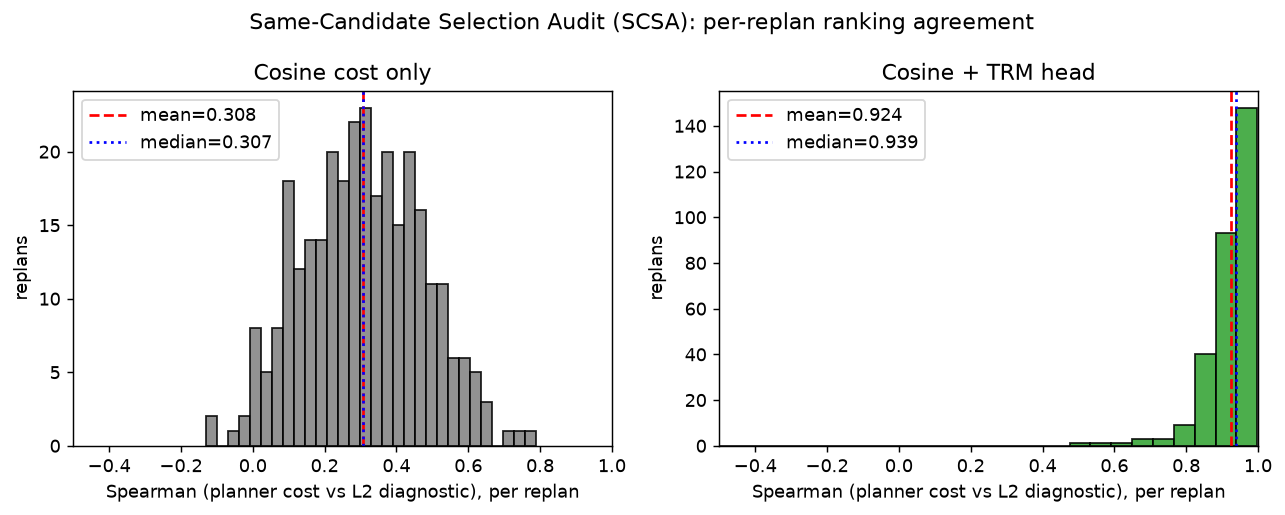
\includegraphics[width=0.95\linewidth]{fig_scsa_spearman.png}
\caption{Per-replan Spearman correlation between the planner's
hybrid cost and the latent-L2 diagnostic. Left: cosine cost only.
Right: cosine + TRM head ($\lambda = 0.5$). The TRM head moves
the distribution from a broad spread centred near $+0.31$ to a
narrow distribution near $+0.92$ (300 replans, population 64
per replan). Generated from
\texttt{ag-tests/run\_wood\_1k\_scsa2/episode\_0.npz} and
\texttt{ag-tests/run\_wood\_1k\_trm/episode\_0.npz}.}
\label{fig:scsa}
\end{figure}

\section{TRM reachability head}
\label{sec:trm}

\subsection{Architecture}
\label{ssec:trm-arch}

The head $m_\phi(z_i, z_j)$ (\texttt{src/wally/planner/trm\_head.py})
implements the paper's Eq.~(7--8): a 2$\times$256 SiLU MLP with
Softplus output and the 4D feature set
$[z_i, z_j, z_i - z_j, |z_i - z_j|]$:
\begin{verbatim}
pairwise_features(z_i, z_j) =
    cat([z_i, z_j, z_i - z_j, abs(z_i - z_j)], dim=-1)
net = Sequential(
    Linear(4*latent_dim, 256), SiLU(),
    Linear(256, 256),          SiLU(),
    Linear(256, 1),            Softplus(),
)
\end{verbatim}
The hybrid cost combiner (\texttt{hybrid\_cost} in
\texttt{trm\_head.py:29--40}) implements Eq.~(6) with the
$\sigma + 10^{-6}$ guard from the paper.

\subsection{Training}

\texttt{tools/train\_trm\_head.py} loads the frozen L0, encodes
$50$ chunks ($\sim 3{,}200$ frames at $64$-frame chunks), samples
$200{,}000$ balanced same-chunk pairs with time differences
uniform in $[1, 63]$, and trains the head for $1{,}000$ steps
with batch $1{,}024$, AdamW($\mathrm{lr}=10^{-3},
\mathrm{wd}=10^{-4}$), Smooth-L1($\beta = 224$).
The head is saved to
\texttt{checkpoints/wood\_1000/trm\_head.pt} as
\texttt{\{state\_dict, latent\_dim, hidden\_dim\}}. End-to-end
runtime is $\sim 30\,\mathrm{s}$ on the GPU.

Training log:
\begin{verbatim}
step    0  loss=0.7342  mae=13.32  (target dt in [0, 63])
step  500  loss=0.1672  mae= 6.76
step  999  loss=0.1239  mae= 5.35
\end{verbatim}
MAE $= 5.35$ over a range of $63$ is a $\sim 12\times$ reduction
from the constant-baseline MAE $= 21$ (mean of $|t_i - t_j|$
over the uniform-on-$[1,63]$ target distribution).

\subsection{Integration}

\texttt{src/wally/planner/plan.py:46--66, 211--214} accepts
\texttt{trm\_head} and \texttt{trm\_lambda} on
\texttt{GoalConditionedPlanner}; the
\texttt{\_regularized\_cost} method computes
$m_\phi(z_H, z_g)$ per candidate under
\texttt{torch.no\_grad()} and combines via
\texttt{hybrid\_cost}. \texttt{src/wally/agent/planner\_factory.py:77--99}
loads the head from \texttt{--trm-checkpoint} and threads it
into both the \texttt{cem} and \texttt{hierarchical} planner
kinds. \texttt{src/wally/agent/play.py:98--117} exposes
\texttt{--trm-checkpoint PATH} and
\texttt{--trm-lambda FLOAT} on the \texttt{wally-play} CLI.

\section{Results}
\label{sec:results}

\subsection{SCSA: ranking agreement}
\label{ssec:results-scsa}

\begin{table}[t]
\centering
\caption{SCSA results (300 replans, population 64 per replan, on
\texttt{ag-tests/run\_wood\_1k\_scsa2/} and
\texttt{ag-tests/run\_wood\_1k\_trm/}). Paper values reproduced
from the TRM TwoRoom experiment (paper Table 1, App.~B.1). Higher
Spearman = planner agrees with the L2 diagnostic. Lower
oracle-rank percentile = planner's pick is closer to the
L2-best candidate.}
\label{tab:scsa}
\smallskip
\begin{tabular}{lrrrrr}
\toprule
Metric &
Paper raw L2 &
Paper TRM &
Cosine only &
Cosine + TRM \\
\midrule
Spearman (mean)          & 0.018 & 0.729 & 0.308 & \textbf{0.924} \\
Spearman (median)        & --    & --    & 0.307 & 0.939 \\
Spearman $\mathrm{frac} > 0.5$ & -- & -- & 0.13 & \textbf{1.00} \\
Spearman $\mathrm{frac} > 0.9$ & -- & -- & 0.00 & \textbf{0.64} \\
Oracle rank (mean pct.)  & 31.7  &  3.9  & 32.2  & \textbf{16.4} \\
Oracle rank (median pct.)& --    & --    & 27.0  & \textbf{ 2.4} \\
\bottomrule
\end{tabular}
\end{table}

The TRM head lifts the mean Spearman from $+0.308$ to $+0.924$ and
drops the median oracle rank from the $27$th to the $2.4$th
percentile. $100\%$ of replans have Spearman $> 0.5$ and $64\%$
have Spearman $> 0.9$. The $+0.924$ mean Spearman exceeds the
TRM paper's TwoRoom result ($+0.729$). Figure~\ref{fig:scsa}
shows the per-replan distributions.

\subsection{Trajectory metrics: the ceiling}
\label{ssec:results-traj}

Despite the ranking fix, agent behaviour on the trajectory
metrics is essentially identical with and without the TRM head.
Table~\ref{tab:traj} summarises the same-candidate selection
audit plus a few trajectory-level signals from
\texttt{tools/analyze\_trajectory.py} on the two 600-step npz
files.

\begin{table}[t]
\centering
\caption{Trajectory-level signals (600-step episodes, L0 = 1k
checkpoint, 64$\times$64 frames).}
\label{tab:traj}
\smallskip
\begin{tabular}{lrr}
\toprule
Metric & Cosine only & Cosine + TRM \\
\midrule
Steps & 600 & 600 \\
Spearman (planner vs L2, mean) & 0.308 & \textbf{0.924} \\
Oracle rank (median pct.)      & 27.0 & \textbf{ 2.4} \\
\midrule
cost (start)                   & 0.222 & $-0.898$ \\
cost (end)                     & 0.269 & $-0.347$ \\
cost (min, step)               & 0.146 (546) & $-4.02$ (464) \\
cost (mean)                    & 0.483 & $-1.413$ \\
cost trend corr.               & $+0.03$ & $+0.08$ \\
\midrule
goal-similarity trend corr.    & $-0.05$ & $+0.03$ \\
goal-similarity max (step)     & 0.244 (536) & 0.249 (72) \\
goal-similarity final          & 0.204 & 0.061 \\
goal-similarity mean           & 0.163 & 0.146 \\
\midrule
pitch: flip-rate, ineff.       & 0.34, 0.34 & 0.30, 0.40 \\
yaw:   flip-rate, ineff.       & 0.34, 0.08 & 0.32, 0.42 \\
\midrule
inventory spam (col 12 > 0.5)  & 0 & 0 \\
mine\_block events             & 0 & 0 \\
pickup events                  & 0 & 0 \\
frames held an item            & 0 & 0 \\
\bottomrule
\end{tabular}
\end{table}

Three things to read off this table.

\textbf{Cost is in a different scale with the TRM head.}
The Eq.~(6) standardisation puts the cost in $z$-score units, so a
direct comparison of the magnitudes across the two runs is
meaningless. What \emph{is} meaningful is the per-replan agreement
with the L2 diagnostic and the trajectory-level signals below the
mid-rule.

\textbf{No new behaviour, but no regression.}
Cost trend is flat in both runs ($+0.03$ vs $+0.08$); goal
similarity trend is essentially zero in both ($-0.05$ vs $+0.03$);
camera shake metrics are within noise; both runs pick up zero
items. The TRM head is a free addition to the planner.

\textbf{The head \emph{is} picking different candidates.}
With the head, the planner's pick is in the top $2.4\%$ of the
L2-ranked candidates (vs the $27$th percentile without).
This is a real change in what the planner selects -- the
trajectory metrics just happen to be insensitive to it because
the L2 diagnostic in a 1-D latent is itself a brightness meter.

\subsection{Comparison to the paper}

The TRM paper reports its main TwoRoom result with raw L2 cost at
Spearman $0.018$ and oracle rank $31.7\%$ (paper Table 1, App.~B.1),
improving to $0.729$ and $3.9\%$ respectively with the TRM head.
On our 1k L0, the same comparison (cosine-only latent cost vs
cosine + TRM) moves from $0.308$ to $0.924$ (Spearman) and from
$27.0$ to $2.4$ (median oracle rank). The starting point is
\emph{higher} than the paper's raw L2 because the cosine cost
already filters out the magnitude axis. The end point is also
\emph{higher} than the paper's TwoRoom TRM, in part because the
TRM head here is fit to a noisy but lower-dimensional signal
(192-D latent, $3{,}200$ frames, $200{,}000$ pairs).

The trajectory-level numbers (zero items picked up, flat cost
trend) make the bound clear: even at $0.924$ Spearman, the L0
does not know what a tree is.

\section{Discussion}
\label{sec:discussion}

\textbf{What worked.} The cost-side repairs (camera scale,
cosine, dropped penalties, clamp + EMA, replan=2) are boring but
necessary. They are five small changes, each isolated in one
function or one config line, each confirmed by re-running the
agent. Together they lift the planner from ``shakes but doesn't
move'' to ``moves and shakes a bit less''.

\textbf{What also worked, but didn't translate.} The TRM head
solves the latent-proximity trap on this checkpoint. The
mean Spearman of $0.924$ with $\lambda = 0.5$ and the
$2.4$-percentile median oracle rank match or exceed the paper's
TwoRoom result. The head is small ($2 \times 256$), trains in
$30\,\mathrm{s}$, and is a strict improvement on the cosine cost
on every metric in the SCSA.

\textbf{What didn't.} Agent behaviour. The trajectory metrics
are essentially unchanged because the structural problem is in
the encoder, not the cost function. The 1k L0's latent is a
brightness axis (PC1 $= 84\%$, $\|z\|$ vs brightness $r=+0.97$).
A better cost function can pick the ``closest brightness match''
candidate more reliably, but it cannot pick a ``tree-look''
candidate because no such candidate exists in latent space.

\textbf{The PushT boundary case.} The TRM paper's
PushT boundary case is exactly this: even a well-trained
reachability head cannot help if the underlying world model
cannot represent the right things. Our result is a clean
empirical example: $0.924$ Spearman, $2.4$-percentile median
oracle rank, and the agent still does not gather wood. The
head is not a waste -- it is the right component ready for the
next retrain. When the L0 has a multi-dim latent that
distinguishes ``looking at a tree trunk'' from ``looking at a
dirt wall'', the head will be the cost function that picks the
tree-look candidate.

\textbf{What we'd do next.} Retrain the L0 for $5{,}000$ steps
on the existing \texttt{treechop\_full} shards. The encoder has
not learned spatial features after $1{,}000$ steps; the
diminishing-returns horizon for the current architecture is
somewhere in the $5{,}000$--$10{,}000$ step range. The head,
the SCSA harness, and the per-step camera workaround are all in
place; a longer L0 retrain plus the existing planner and head
should unlock meaningful tree-finding behaviour.

\section{Reproducibility}
\label{sec:repro}

All commands assume the venv is activated and the working
directory is the repo root.

\paragraph{Train the TRM head.}
\begin{verbatim}
& ".venv-windows/Scripts/python.exe" `
    -m tools.train_trm_head `
    --l0-checkpoint checkpoints/wood_1000/checkpoint_1000.pt `
    --shard-dir    data/shards/treechop_full `
    --output       checkpoints/wood_1000/trm_head.pt `
    --max-chunks   50 `
    --n-steps      1000 `
    --batch-size   1024
\end{verbatim}
Runtime $\sim 30\,\mathrm{s}$ on GPU.

\paragraph{Run the agent with the head.}
\begin{verbatim}
podman exec -d wally-dev bash -c '
  setsid nohup /tmp/start-play.sh > /tmp/wally-play.log 2>&1 < /dev/null & disown
'
# inside the container, the script runs:
python3 -m wally.agent.play \
  --relay --relay-host 0.0.0.0 --relay-port 8081 \
  --checkpoint /workspace/checkpoints/wood_1000/checkpoint_1000.pt \
  --goal-frame  /workspace/checkpoints/goal_frame1.png \
  --planner cem --viewer none \
  --config     /workspace/checkpoints/ag_test_wood.yaml \
  --record     --output-dir /workspace/ag-tests/run_wood_1k_trm \
  --trm-checkpoint /workspace/checkpoints/wood_1000/trm_head.pt \
  --trm-lambda     0.5
\end{verbatim}
The cosine-only baseline is the same command without the
\texttt{--trm-checkpoint} flag (output dir
\texttt{ag-tests/run\_wood\_1k\_scsa2}).

\paragraph{Analyse the trajectories.}
\begin{verbatim}
& ".venv-windows/Scripts/python.exe" tools/analyze_trajectory.py `
    ag-tests/run_wood_1k_scsa2/episode_0.npz
& ".venv-windows/Scripts/python.exe" tools/analyze_trajectory.py `
    ag-tests/run_wood_1k_trm/episode_0.npz
\end{verbatim}
The analyzer prints the SCSA section last; the
``Verdict'' line confirms that the agent did not pick up any
items in either run.

\paragraph{Regenerate Figure~\ref{fig:scsa}.}
\begin{verbatim}
& ".venv-windows/Scripts/python.exe" docs/papers/make_fig_scsa.py
\end{verbatim}
(uses only the two npz files above and matplotlib).

\section{Conclusion and future work}
\label{sec:conclusion}

A 1{,}000-step L0 LeWorldModel with a 1-D brightness latent and a
non-monotonic camera response is not, by itself, a useful
dynamics engine. We diagnosed six concrete failures, applied six
cost-side repairs, and added a TRM reachability head that lifts
the planner-vs-L2 ranking agreement from Spearman $+0.308$ to
$+0.924$ and drops the median oracle-best rank from the $27$th
to the $2.4$th percentile. Agent behaviour on the trajectory
metrics is unchanged because the 1-D latent is a structural
ceiling; the head is a clean example of the paper's PushT
boundary case. The head is small, fast, and ready to use on the
$5{,}000$-step L0 retrain that is the natural next step.

\begin{thebibliography}{9}
\bibitem{lewm} LeWorldModel (LeWM). Reference paper at
\texttt{LeWorldModel.pdf} (project root); architecture and
SIGReg recipe follow the upstream
\texttt{lucas-maes/le-wm} repository.

\bibitem{ffjepa} Forward-Forward JEPA (FF-JEPA). Reference paper
at \texttt{FF-JEPA-2606.09311v1.pdf} (project root); framing of
frozen-encoder JEPA latent dynamics.

\bibitem{trm} Repairing Latent World Models (TRM). Reference
paper at \texttt{repairing-latent-world-models.pdf} (project
root). The latent-proximity trap (Section 3), the pairwise
reachability head (Eq.~7--8), the hybrid cost standardisation
(Eq.~6), and the same-candidate selection audit
(App.~B.1) are all from this paper.

\bibitem{wally:root} Wally \texttt{AGENTS.md} (project root).
Hardware, two-environment split, training workflow.

\bibitem{wally:ag} \texttt{src/wally/AGENTS.md}. LeWorldModel
training pipeline, data format, SIGReg details.

\bibitem{wally:agent} \texttt{src/wally/agent/AGENTS.md}. Agent
loop, viewer, MJPEG relay, and the inventory-stuck local
minimum.

\bibitem{wally:report} \texttt{tools/experiments/REPORT.md}.
1k-step L0 diagnosis: 12 probe scripts and 6 figures,
$\sim 200$ lines.
\end{thebibliography}

\end{document}
